\documentclass[../hw5]{subfiles}
\begin{document}
\begin{problem}[4]
Let $S\subset \R^3$ be defined by $x^2 - 4y^2 + z^2=1$. Let $p=(0,0,5)$.
\begin{enumerate}[label=(\alph*)]
	\item Find $x \in S$ closest to $p$, or prove there is no such $x$.
	\item Find $x \in S$ furthest from $p$, or prove there is no such $x$.
	\item Sketch $S$ supporting answers to parts  $a$ and  $b$.
\end{enumerate}
\end{problem}
\begin{proof}[Proof of a]
	We will use $f(x,y,z)=x^2 + y^2 + {(z-5)}^2$ to give the distance squared from $p$. We will minimize $f$ with respect to $g(x,y,z)=x^2 - 4y^2 + z^2 - 1$.

	So, $\nabla f = (2x,2y,2z-10)$ and $\nabla g = (2x,-8y,2z)$. Then, $\nabla f = \lambda \nabla g \implies$
	\begin{align*}
		2x    = 2\lambda x  & \implies x=0 \lor \lambda = 1    \\
		2y    = -8\lambda y & \implies y=0 \lor \lambda = -1/4 \\
		2z-10 = 2\lambda z  & \implies z = \frac{5}{1-\lambda}
		.\end{align*}

	If $\lambda=1$, then  $z$ is of indeterminate form.
	So we must have $x=0$.
	For the first case, we will consider $\lambda=-\frac{1}{4}$, which gives $z=4$.
	But, our constraint $g$ and $x=0$ provide that $-4y^2 + 4^2 = 1$, so $y^2=\frac{15}{4} \implies y= \frac{\pm \sqrt{15}}{2}$.
	Thus, we have a critical point at $\left(0,\frac{ \pm \sqrt{15} }{2},4\right)$.

	For the second case, we will use $y=0$, yet, with our constraint  $g$ and  $x=0$, then  $z^2=1\implies z= \pm 1$. So we also have critical points $(0,0, \pm 1)$.
	Evaluating $f$ at these critical points yields,
	\begin{align*}
		f(0,0,1)                                  & = 16           \\
		f(0,0,-1)                                 & = 36           \\
		f\left(0,\frac{\pm \sqrt{15}}{2},4\right) & = \frac{19}{4}
		.\end{align*}

	So, the minimum distance squared is $\frac{19}{4}$.
	Thus, the point of $S$ closest to $p$ is $\left( 0,\frac{\pm\sqrt{15}}{2}  \right) $, at $\frac{\sqrt{19}}{2}$ units away.
\end{proof}
\begin{proof}[Proof of b]
	Since $S$ is a hyperboloid of one sheet, then  there is no point on $S$ furthest from  $p$.
\end{proof}

\begin{figure*}[h]
	\centering
	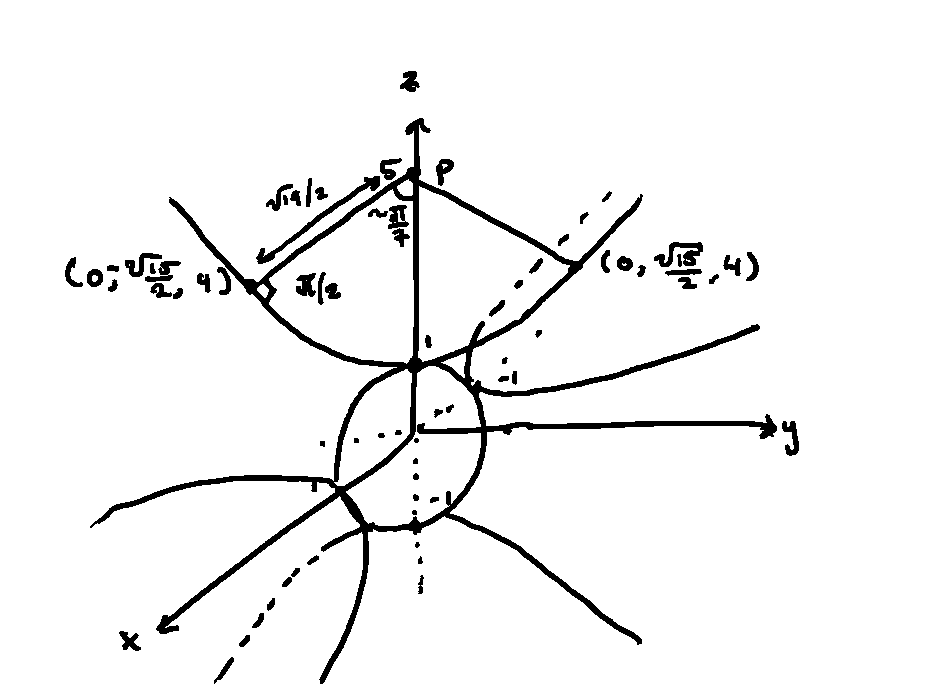
\includegraphics[width=0.6\textwidth]{figures/handdrawn_figure.pdf}
	\caption{Sketch of $S\subset \R^3$}
\end{figure*}

\end{document}
